\chapter{Implementierung von Reforge}

\section{Entwicklung des Backends}
Das Backend von \textit{Reforge} ist für die Verarbeitung der hochgeladenen Dateien und die Generierung der technischen Berichte verantwortlich. 


\subsection{Kommunikation zwischen Frontend und Backend}
\label{subse:kommu_froback}

Es wird nun im folgendem die Kommunikation zwischen Frontend und Backend von \textit{Reforge} näher erläutert. Ziel dieser Kommunikation ist der Austausch von Daten und die Bereitstellung eines verarbeiteten Berichts als Datei-Download für den Benutzer. Der Ablauf erfolgt mit einer RESTful \ac{API}. Er wird erst gestartet, sobald der Nutzer im Frontend zum Beispiel einen LaTeX-ZIP-Ordner einfügt, alle nötigen Parameter ausfüllt und auf den Button \textbf{Start the generation} klickt.

Das Listing \ref{lst:Frontend_API_Aufruf} zeigt den Code für den Aufruf der RESTful \ac{API} im Frontend. Die \ac{URI} \texttt{http://localhost:5000/api/upload} verweist auf den Endpunkt des Backends, der für das Hochladen von Dateien zuständig ist. Die Anfrage wird als \ac{HTTP} \textbf{POST} gesendet, da Dateien und zusätzliche Parameter wie das gewünschte Format oder die Sprache übermittelt werden. Der Header \texttt{Content-Type} ist auf \texttt{multipart/form-data} gesetzt, um dem Server mitzuteilen, dass es sich um einen Datei-Upload handelt. Zusätzlich wird mit \texttt{responseType: 'blob'} spezifiziert, dass die Antwort vom Server als \ac{Blob} erwartet wird, was für den späteren Download des Berichts wichtig ist. Es dient unter anderem dazu, binäre Daten übertragbar zu machen. So ist es möglich, die Dateien später herunterzuladen.


\begin{listing}[H]
\begin{minted}[
frame=lines,
bgcolor=base,
fontsize=\footnotesize,
linenos
]
{typescript}
// API-Aufruf im Frontend
const response = await axios.post('http://localhost:5000/api/upload', formData, {
  headers: {
    'Content-Type': 'multipart/form-data',
  },
  responseType: 'blob',
});
\end{minted}
\caption{API POST Aufruf im Frontend}
\label{lst:Frontend_API_Aufruf}
\end{listing}

Nachdem das Backend die Anfrage erhalten hat, wird die hochgeladene Datei verarbeitet. Sobald das Backend alle Verarbeitungsschritte zur Erstellung des Berichts abgeschlossen hat, fügt es die neuen Informationen in den Header der Antwort ein. Der Statuscode 200 wird zurückgesendet, um anzuzeigen, dass die Anfrage des Frontends erfolgreich verarbeitet wurde. Gleichzeitig wird der zusammengesetzte Bericht mit dem Statuscode an das Frontend gesendet. Das folgende Listing \ref{lst:Backend_API_Antwort} zeigt, wie der Code dafür aussieht.

\begin{listing}[H]
\begin{minted}[
frame=lines,
bgcolor=base,
fontsize=\footnotesize,
linenos
]
{typescript}
// API-Antwort im Backend
    res.setHeader('Content-Disposition', `attachment; filename="${title}.tex"`);
    res.setHeader('Content-Type', 'text/plain');
    res.status(200).send(combinedReport);
\end{minted}
\caption{Zurücksendung der abgeschlossenen \ac{API}-Anfrage ans Frontend}
\label{lst:Backend_API_Antwort}
\end{listing}

Im Frontend wird die Antwort des Backends überprüft, wie in Listing \ref{lst:Frontend_API_Antwort} dargestellt. Bei einem Statuscode von \texttt{200} wird ein neues \texttt{\ac{Blob}}-Objekt erzeugt, das die empfangenen Binärdaten (\texttt{combinedReport}) enthält. Mithilfe von \texttt{window.URL.createObjectURL} wird eine \ac{URL} generiert, die es dem Benutzer ermöglicht, die Datei herunterzuladen.

\begin{listing}[H]
\begin{minted}[
frame=lines,
bgcolor=base,
fontsize=\footnotesize,
linenos
]
{typescript}
if (response.status === 200) {
  const url = window.URL.createObjectURL(new Blob([response.data]));
  setUploadStatus('File successfully uploaded.');

  navigate('/download', { state: { downloadUrl: url, title: title, format: format } });
} else {
  setUploadStatus('Error while uploading the file.');
}
\end{minted}
\caption{API Rückgabe Empfang im Frontend}
\label{lst:Frontend_API_Antwort}
\end{listing}

Die \ac{URL}-Generierung erfolgt dabei in mehreren Schritten. Zunächst wird das vom Backend empfangene Binärdatenobjekt als \texttt{\ac{Blob}} formatiert.  Anschließend wird mit \texttt{window.URL.createObjectURL(blob)} eine temporäre \ac{URL} erstellt, die im Browser als Verweis auf dieses \ac{Blob} dient. Diese \ac{URL} ist nur während der aktuellen Browsersitzung gültig und sieht beispielsweise so aus:

\texttt{blob:http://localhost:3000/3f9a8d7e-2b4c-48e6-a91f-bb23c1def456}. 

Nach der \ac{URL}-Erstellung wird der Benutzer auf eine neue Seite weitergeleitet, auf der er den Bericht herunterladen kann. Ist hingegen vorher ein Fehler aufgetreten, beispielsweise wenn das Backend einen anderen Statuscode zurückgibt, wird statt der Weiterleitung eine Fehlermeldung angezeigt.

Auf diese Weise wird die gesamte Kommunikation zwischen Frontend und Backend durch einen einzigen \textbf{POST}-Request ermöglicht. Das Frontend überträgt alle notwendigen Informationen an das Backend und wartet auf die Antwort. Nach erfolgreicher Verarbeitung stellt das Backend den generierten Bericht als Datei bereit, die im Frontend heruntergeladen werden kann. 

\subsection{Verwendete Backend Bibliotheken}
Die Backend-Entwicklung der Anwendung basiert auf einer Reihe von Bibliotheken, die die Verarbeitung von Daten, die Dateiverwaltung und die Bereitstellung der \ac{API}s unterstützen. Im Folgenden werden die verwendeten Bibliotheken aus dem Listing \ref{lst:Backend_Bibliotheken} und ihre Hauptfunktionen beschrieben.

\begin{listing}[H]
\begin{minted}[
frame=lines,
bgcolor=base,
fontsize=\footnotesize,
linenos
]
{typescript}
"dependencies": {
    "adm-zip": "^0.5.15",
    "bottleneck": "^2.19.5",
    "cors": "^2.8.5",
    "docx": "^8.5.0",
    "express": "^4.17.1",
    "jsdom": "^25.0.1",
    "multer": "^1.4.2"
}
\end{minted}
\caption{Backend Bibliotheken}
\label{lst:Backend_Bibliotheken}
\end{listing}

Die Bibliothek ADM-ZIP ermöglicht den einfachen Umgang mit ZIP-Dateien. Sie dient zum Erstellen, Entpacken und Lesen von ZIP-Archiven. Da in Reforge mit LaTeX-ZIP-Dateien gearbeitet wird, ist diese Bibliothek unverzichtbar.

Die Bottleneck-Bibliothek wird für die Verwaltung von Anforderungsraten verwendet. Sie hilft, die Anzahl der gleichzeitigen Anfragen an externe \ac{API}s zu kontrollieren, um eine Überlastung zu vermeiden.

Die CORS Bibliothek ermöglicht die Aktivierung von \ac{CORS}, um den Zugriff von Webanwendungen auf Serverressourcen zu kontrollieren. Dies ist notwendig, damit der Frontend-Client sicher auf die Backend-Ressourcen zugreifen kann.

Die \ac{DOCX}-Bibliothek wird zur Erzeugung von Word-Dokumenten verwendet. Sie ermöglicht es der Anwendung, Berichte im Word-Format zu erstellen und diese zu formatieren.

Express ist ein minimalistisches Web-Framework für Node.js, das die Entwicklung von Backend-Servern vereinfacht. Es bietet Funktionen zur Erstellung von \ac{API}s, die das Rückgrat der serverseitigen Logik bilden. Express stellt sicher, dass die Kommunikation zwischen Client und Server reibungslos verläuft.

Die jsdom-Bibliothek bietet eine JavaScript-Implementierung des \ac{DOM}. Sie ermöglicht das Parsen und Manipulieren von \ac{HTML} im Backend, was bei der Verarbeitung und Extraktion von Daten aus \ac{DOCX}-Dokumenten hilfreich ist.

Multer ist eine Middleware für Datei-Uploads. Sie wird verwendet, um die vom Benutzer hochgeladenen Dateien zur Verarbeitung entgegenzunehmen. Diese Dateien werden mit der Funktion \textbf{memoryStorage()} im Arbeitsspeicher zwischengespeichert. Diese Bibliotheken bilden die Grundlage für das Backend von \textit{Reforge}.

\subsection{LaTeX-ZIP-Verarbeitung}

In diesem Abschnitt werden die einzelnen Prozessschritte der LaTeX-ZIP-Verarbeitung erläutert. Im Listing \ref{lst:Entscheidung_ZIP_DOCX} ist zu sehen, wie das Backend zunächst prüft, ob es sich bei der hochgeladenen Datei um eine ZIP-Datei handelt. Abhängig davon wird hier entweder der ZIP-Prozess oder der \ac{DOCX}-Prozess gestartet.

\begin{listing}[H]
\begin{minted}[
frame=lines,
bgcolor=base,
fontsize=\footnotesize,
linenos
]
{typescript}
if (req.file.originalname.endsWith('.zip')) {
  combinedReport = await processZipFile(req.file, mainfile, author, language, format);
} else if (req.file.originalname.endsWith('.docx')) {
  combinedReport = await processDocxFile(req.file, author, language, format);
}
\end{minted}
\caption{Entscheidung zwischen der ZIP- oder \ac{DOCX}-Verarbeitung}
\label{lst:Entscheidung_ZIP_DOCX}
\end{listing}

LaTeX-Projekte sind häufig in mehrere Kapitel und Abschnitte unterteilt, die in separaten Dateien organisiert sind. Diese Struktur wird durch die Hauptdatei gesteuert, in der die einzelnen Kapiteldateien mittels \texttt{\textbackslash include\{\}}-Anweisungen eingebunden werden. Um die korrekte Reihenfolge der Kapitel für die Weiterverarbeitung zu haben, muss die Reihenfolge dieser \texttt{include}-Anweisungen aus der Hauptdatei entnommen werden. Damit die spätere Zusammenfassung in der richtigen Reihenfolge erfolgt, ist dieser Schritt unerlässlich.

Im Frontend fragt die Anwendung über einen Parameter den Namen der Hauptdatei des LaTeX-Ordners ab. Das Listing \ref{lst:Mainfile_Search} zeigt den Code für die Suche nach der Hauptdatei. Sobald also die Funktion \textbf{processZipFile} aufgerufen wird, wird zunächst geprüft, ob die angegebene Hauptdatei innerhalb des ZIP-Ordners gefunden werden kann. Wenn die Hauptdatei nicht gefunden werden kann, wird ein Fehler ausgegeben. Ist die Suche nach der Hauptdatei erfolgreich, wird mit der Funktion \textbf{getIncludeOrder} jede Include-Anweisung in einem String gespeichert. Außerdem wird hier die ADM-ZIP Bibliothek verwendet, um die ZIP-Inhalte zu durchsuchen und die Dateien zu entnehmen.

\begin{listing}[H]
\begin{minted}[
frame=lines,
bgcolor=base,
fontsize=\footnotesize,
linenos
]
{typescript}
  const zip = new AdmZip(file.buffer);
  const zipEntries = zip.getEntries();
  const path = require('path');
  let includeOrder: string[] = [];
  let mainFileFound = false;

  // Mainfile im zip finden
  for (const zipEntry of zipEntries) {
    const entryName = path.basename(zipEntry.entryName);
    
    // wenn mainfile gefunden -> hole include reihenfolge
    if (!zipEntry.isDirectory && entryName === mainfile) {
      mainFileFound = true; 
      const fileContent = zipEntry.getData().toString('utf-8');
      if (fileContent.includes('\\include{')) {
        includeOrder = getIncludeOrder(fileContent);
        break;
      }
    }
  }
  
  // error wenn mainfile nicht gefunden
  if (!mainFileFound) throw new Error(`Main file "${mainfile}" not found in ZIP`);
\end{minted}
\caption{Dieser Codeabschnitt sucht die LaTeX-Hauptdatei im ZIP-Ordner und holt sich die Include-Reihenfolge aus der Hauptdatei}
\label{lst:Mainfile_Search}
\end{listing}

\subsubsection{Die getIncludeOrder-Funktion}

Der folgende Code in Listing \ref{lst:getIncludeORder} zeigt die Implementierung der Funktion, welche die Include-Reihenfolge ausliest. Die Suche nach dem Inhalt erfolgt mit einem regulären Ausdruck, wobei der Inhalt zwischen den geschweiften Klammern \texttt{\{\}} des regulären Ausdrucks am wichtigsten ist, da wir diesen Inhalt für die Datei zusammenstellung benötigen. Dieser Part des Musters wird dementsprechend näher erläutert: \texttt{([\textasciicircum\}]+)}

\begin{listing}[H]
\begin{minted}[
frame=lines,
bgcolor=base,
fontsize=\footnotesize,
linenos
]
{typescript}
function getIncludeOrder(mainfile: string): string[] {
  const includePattern = /\\include\{([^}]+)\}/g;
  let match;
  const includeFiles: string[] = [];
  
  //suche nach Übereinstimmungen solange match !== null 
  while ((match = includePattern.exec(mainfile)) !== null) {
    //jedes gefundene include wird in den array gepushed
    includeFiles.push(match[1].trim());
  }

  return includeFiles;
}
\end{minted}
\caption{Funktion zur Extraktion der Include-Reihenfolge}
\label{lst:getIncludeORder}
\end{listing}

Für ein besseres Verständnis wird das Muster \texttt{([\textasciicircum\}]+)} in mehreren Teilen erklärt. Die eckigen Klammern \texttt{[\textasciicircum\}]} definieren eine Negation. Das \texttt{\textasciicircum} bedeutet \glqq nicht \grqq{}, also steht \texttt{[\textasciicircum\}]} für \glqq kein \}\grqq{}. Das Pluszeichen \texttt{+} bedeutet, dass mindestens ein oder mehrere Zeichen gefunden werden sollen, die nicht \texttt{\}} sind. Die runden Klammern \texttt{(...)} um \texttt{([\textasciicircum\}]+)} gruppieren diesen Teil und sorgen dafür, dass der Inhalt in einer sogenannten Capture Group gespeichert wird. Mit diesem Muster können alle Dateinamen innerhalb der Include-Klammer extrahiert werden.

Solange das Muster in der While-Schleife Übereinstimmungen findet, wird diese Übereinstimmung in einem String angelegt. Dazu wird mit \texttt{match[1]} auf den gefundenen Inhalt der Capture Group zugegriffen. Zusätzlich wird mit \texttt{trim()} sichergestellt, dass keine unerwünschten Leerzeichen enthalten sind.

\subsubsection{Kombinieren der Kapiteldateien}

Nachdem die Reihenfolge der Kapiteldateien ermittelt wurde, müssen die entsprechenden \texttt{.tex}-Dateien aus dem ZIP-Archiv geladen und in der richtigen Reihenfolge zusammengefügt werden. Das folgende Listing \ref{lst:Kombination der Kapiteldateien} zeigt, wie die Dateien aus dem ZIP-Archiv mit der erhaltenen Reihenfolge zusammengefügt werden.

\begin{listing}[H]
\begin{minted}[
frame=lines,
bgcolor=base,
fontsize=\footnotesize,
linenos
]
{typescript}
for (const fileName of includeOrder) {
  //hinzufügen von .tex  zur filename falls nicht vorhanden
  const texFileName = fileName.endsWith('.tex') ? fileName : `${fileName}.tex`;
  //finde texFileName im Zip
  const zipEntry = zipEntries.find(entry => entry.entryName.endsWith(texFileName));
  //prüfung ob datei existiert und kein verzeichnis ist
  if (zipEntry && !zipEntry.isDirectory) {
    //hole text inhalt
    let fileContent = zipEntry.getData().toString('utf-8');
    //sammlung von allen datei inhalten in allFileContent
    allFileContent += fileContent + '\n';
  }
}
\end{minted}
\caption{Kombination der Kapiteldateien}
\label{lst:Kombination der Kapiteldateien}
\end{listing}

Zunächst wird geprüft, ob der Dateiname die Endung \texttt{.tex} enthält. Falls nicht, wird diese angehängt, da in LaTeX-Dateien oft nur der Basisname im Include angegeben ist. Anschließend wird das ZIP-Archiv nach der entsprechenden Datei durchsucht. Wenn die Datei gefunden wird und es sich nicht um ein Verzeichnis handelt, wird ihr Inhalt ausgelesen und in der Variablen \texttt{allFileContent} gespeichert. Dieses Verfahren stellt sicher, dass die Kapiteldateien in der richtigen Reihenfolge kombiniert werden, so dass der gesamte Text des Dokuments vollständig rekonstruiert werden kann.

\subsubsection{LaTeX-Textfilter und Aufteilung}

Um sicherzustellen, dass nur die relevanten Teile eines LaTeX-Dokuments an die OpenAI-Schnittstelle für die Erstellung von Zusammenfassungen übergeben werden, ist es notwendig, den Text vorher zu bereinigen. Außerdem ist die Anzahl der übertragbaren Token begrenzt, so dass überflüssige LaTeX-Befehle, Kommentare und unnötige Leerzeichen aus dem Text entfernt werden müssen. Der Befehl \texttt{\textbackslash chapter} bleibt jedoch erhalten, da dieser für die spätere Aufteilung des Textes wichtig ist. Für die Filterung werden reguläre Ausdrücke verwendet, um LaTeX-Kommandos gezielt auszusortieren beziehungsweise beizubehalten. Ein Codeauszug der LaTeX-Filterfunktion ist im Anhang im Listing \ref{lst:LaTeX-Text-Filterung} zu finden. 

Auch nach der Filterung ist der Gesamttext noch zu lang, so dass eine sinnvolle Zerlegung des Dokuments notwendig ist. Damit die \ac{KI} sinnvolle Zusammenfassungen erstellen kann, ohne den Kontext zu verlieren, wird der Text mit Hilfe der \texttt{\textbackslash chapter}-Kommandos zerlegt. Aus diesem Grund wurden die \texttt{\textbackslash chapter}-Befehle vorher nicht herausgefiltert. Diese Vorgehensweise ermöglicht es, die begrenzte Anzahl von Token der OpenAI einzuhalten und dennoch einen zusammenhängenden Text für die Zusammenfassungen zu erzeugen. Die Kapitelaufteilung ist im Listing \ref{lst:Chapter_Mapping} in Zeile zwei dargestellt.

\begin{listing}[H]
\begin{minted}[
frame=lines,
bgcolor=base,
fontsize=\footnotesize,
linenos
]
{typescript}
//Zerstückelung des Textes bei Chapter
const chapters = allFileContent.split(/(?=\\chapter\{)/g);

//Alle Kapitel durchgehen & Bericht erstellen
const reportPromises = chapters.map((chunk) => {
  const chapternameMatch = chunk.match(/\\chapter\{([^}]+)\}/); 
  const chapterTitle = chapternameMatch ? chapternameMatch[1] : 'Unnamed Chapter'; 
    
  return LanguageDetection(chunk, language, author, format, 'tex').then((report) => {
    return `\\section{${chapterTitle}}\n${report}`;
  });
});
const reportParts = await Promise.all(reportPromises);
let combinedReport = reportParts.join('\n\n');
 
combinedReport = removeSpecialChars(combinedReport);
\end{minted}
\caption{Chapter-Mapping für die Textübertragung an OpenAI}
\label{lst:Chapter_Mapping}
\end{listing}

Darüber hinaus wird im Listing \ref{lst:Chapter_Mapping} ein Kapitel-Mapping durchgeführt, damit jedes einzelne Kapitel für die Zusammenfassungsgenerierung übergeben wird. Um sicherzustellen, dass die Kapitelnamen während des Prozesses nicht verloren gehen, werden diese zuvor mit einem regulären Ausdruck gesucht und in \texttt{ChapterTitle} abgelegt. Ist kein Titel vorhanden, wird der Textabschnitt mit \texttt{Unnamed Chapter} betitelt. In der Funktion \textbf{Language Detection} findet die Spracherkennung und die Kommunikation mit OpenAI statt. Diese Funktion wird im folgenden Abschnitt erläutert. Anschließend werden alle generierten Berichtsteile wieder in \texttt{combinedReport} zusammengeführt.

Es kann vorkommen, dass OpenAI bei der Generierung Sonderzeichen wie \& oder \% verwendet. Da LaTeX mit solchen Zeichen Fehler aufwirft, werden diese mit der Funktion \textbf{removeSpecialChars} nachträglich entfernt. Zusätzlich entfernt diese Funktion die ursprüngliche Nummerierung der Überschriften. Diese Funktion ist im Listing \ref{lst:SpecialChar-Filterung} im Anhang zu finden.

\subsubsection{Die LanguageDetection-Funktion}
Die von OpenAI generierten Texte wurden nicht immer zuverlässig in der richtigen Sprache zurückgegeben, obwohl im Prompt die gewünschte Sprache angegeben wurde. Um dieses Problem zu lösen, wurde eine Spracherkennung implementiert, welche die Sprache des generierten Textes mit der gewünschten Sprache vergleicht.

Das Listing \ref{lst:dowhile_LanguageDetection} zeigt den Teil der Funktion \textbf{Language Detection}, in dem eine Schleife ausgeführt wird, bis die erkannte Sprache im generierten Bericht mit der erwarteten Sprache übereinstimmt. Im Frontend kann der Benutzer auswählen, ob die Ausgabe in Englisch oder Deutsch erfolgen soll. Diese Auswahl wird als \textit{erwartete Sprache} definiert. Nur wenn die Sprachen übereinstimmen, wird der in \textbf{generateTechReport} erzeugte Bericht zurückgegeben. Die Spracherkennung erfolgt über die Funktion \textbf{detectLanguageUsingStopWords}, welche die Sprache der generierten Texte anhand von Stopwörtern überprüft. Wie die Spracherkennung mittels Stopwörtern funktioniert, wird im folgenden Abschnitt erläutert.

\begin{listing}[H]
\begin{minted}[
frame=lines,
bgcolor=base,
fontsize=\footnotesize,
linenos
]
{typescript}
do {
  summary = await generateTechReport(content, expectedLanguage, format, docType);

  detectedLanguage = detectLanguageUsingStopWords(summary);
    
  if (detectedLanguage.toLowerCase() !== expectedLanguage.toLowerCase()) {
    console.log(`Sprache nicht korrekt erkannt. Versuche erneut...`);
  }
} while (detectedLanguage.toLowerCase() !== expectedLanguage.toLowerCase());
  return summary;
}
\end{minted}
\caption{Do-While-Schleife der LanguageDetection-Funktion}
\label{lst:dowhile_LanguageDetection}
\end{listing}

\subsection{Spracherkennung mittels Stopwörtern}

Die Analyse von Stoppwörtern ist eine einfache Methode, um die Sprache eines Textes zu ermitteln. Stoppwörter sind Wörter, die in der natürlichen Sprache als wenig informativ gelten und häufig vorkommen. Sie können jedoch Hinweise auf die Sprache eines Textes geben, da ihre genaue Form von Sprache zu Sprache variiert.

Dunning hat gezeigt, dass statistische Methoden zur Spracherkennung eingesetzt werden können. Die Idee dahinter ist, dass man anhand der Verteilung von Zeichenketten feststellen kann, ob ein Text beispielsweise auf Deutsch oder Englisch verfasst wurde \cite{dunning1994statistical}. Bei diesem Ansatz werden statt Zeichenketten Stoppwörter verwendet, um die Sprachverteilung zu bestimmen.

\subsubsection{Warum sind Stopwörter nützlich für die Spracherkennung?}
\begin{itemize}
    \item \textbf{Hohe Häufigkeit und Sprachspezifität:}  
    Stopwörter treten in jedem Text häufig auf, ihre Form ist jedoch in jeder Sprache unterschiedlich. Beispielsweise kommen die deutschen Stopwörter \glqq der\grqq{}, \glqq die\grqq{}, \glqq das\grqq{} oft in deutschen Texten vor, während sie in englischen Texten fehlen. Umgekehrt finden sich englische Stopwörter wie \glqq the\grqq{}, \glqq and\grqq{}, \glqq is\grqq{} in fast jedem englischen Text.

    \item \textbf{Geringe Bedeutung für den Inhalt:}  
    Da Stoppwörter eher eine grammatische als eine inhaltliche Funktion haben, kommen sie in fast allen Texten vor. Dies ermöglicht es, die Sprache eines Textes zu identifizieren, ohne den Inhalt genauer analysieren zu müssen.

    \item \textbf{Effizienz:}  
    Die Spracherkennung mittels Stoppwörtern ist sparsam, da nur eine kleine Gruppe von Wörtern gesucht und deren Häufigkeit gezählt wird. Dies ermöglicht eine schnelle Sprachanalyse.
\end{itemize}

\subsubsection{Begrenzungen dieser Methode}

Bei mehrsprachigen Texten kann es schwierig sein, eine klare Sprache zu definieren. Außerdem können kurze Texte zu einem Mangel an Stoppwörtern führen. Ähnliche Sprachen wie Spanisch und Portugiesisch können ebenfalls zu Unterscheidungsschwierigkeiten beitragen. Diese Einschränkungen gelten jedoch nicht für \textit{Reforge}, da die Dateneingabe beispielsweise aus Bachelorarbeiten besteht. Diese sind in der Regel ausreichend lang und nur in einer Sprache verfasst. 

\subsubsection{Die in \textit{Reforge} verwendeten Stopwörter:}

\begin{listing}[H]
\begin{minted}[
frame=lines,
bgcolor=base,
fontsize=\footnotesize,
linenos
]
{typescript}
const englishStopWords = ["the", "as", "by", "of", "is", "and"];
const germanStopWords = ["der", "die", "das", "von", "ist", "und"];
\end{minted}
\caption{Verwendete Stopwörter in Reforge}
\label{lst:stopwords}
\end{listing}

\subsubsection{Implementierung der Spracherkennung mittels Stopwörtern}

Um die Sprache eines Textes zu bestimmen, wird der Text auf das Vorkommen der in Listing \ref{lst:stopwords} aufgeführten Stopwörter untersucht. Der dazu notwendige Algorithmus ist in Listing \ref{lst:stopwords_funktion} dargestellt.  Dabei wird für jedes gefundene Stopwort der entsprechende Zähler für die jeweilige Sprache erhöht. Am Ende vergleicht man die Zählerwerte. Ist der deutsche Zähler höher, so handelt es sich um einen deutschsprachigen Text. Ist der englische Zähler höher, liegt ein englischsprachiger Text vor. Sollte es jedoch zu einem Unentschieden kommen, kann die Sprache nicht eindeutig bestimmt werden, und es wird Unknown zurückgegeben. Dies kann darauf hindeuten, dass der Text entweder in keiner der beiden Sprachen verfasst wurde oder eine Mischung aus Deutsch und Englisch enthält.

\begin{listing}[H]
\begin{minted}[
frame=lines,
bgcolor=base,
fontsize=\footnotesize,
linenos
]
{typescript}
function detectLanguageUsingStopWords(text: string): string{
  const words = text.toLowerCase().split(/\s+/);
  
  let englishCount = 0;
  let germanCount = 0;

  words.forEach(word => {
    if (englishStopWords.includes(word)) {
      englishCount++;
    }
    if (germanStopWords.includes(word)) {
      germanCount++;
    }
  });

  if (englishCount > germanCount) {
    return "english";
  } else if (germanCount > englishCount) {
    return "deutsch";
  } else {
    return "Unknown";
  }
}
\end{minted}
\caption{Spracherkennungsverfahren mit Stopwörtern}
\label{lst:stopwords_funktion}
\end{listing}

\subsection{OpenAI und DeepL}

\subsubsection{Der OpenAI \ac{API} Aufruf für die Textgenerierung}
Um eine automatische Zusammenfassung für die Dokumente zu erstellen, wird die OpenAI \ac{API} verwendet. Dafür wird ein \ac{API}-Aufruf durchgeführt, welcher die Texte an das \ac{GPT}-3.5-Turbo Modell von OpenAI übermittelt. Dort werden die Texte zusammengefasst und in der entsprechenden Sprache zurückgeliefert.

Die \ac{API}-Anfrage hierfür ist im Listing \ref{lst:OpenAI-Request} dargestellt. Hier wird der Inhalt mit einem \textbf{POST} an die \ac{URI} von OpenAI gesendet. Zum besseren Verständnis der Verarbeitung müssen in diesem Request jedoch noch zusätzliche Informationen angegeben werden. Wie bereits in Kapitel \ref{4.3_LLM} erwähnt, muss angegeben werden, welches Modell OpenAI für die Anfrage verwenden soll. Außerdem muss angegeben werden, welche Nachricht an das Model übergeben werden soll. Diese Nachricht ist in zwei Rollen aufgeteilt. Die Rolle des Systems und die Rolle des Benutzers. Für die Benutzerrolle wird der erstellte Prompt eingefügt. Der Prompt enthält den Textinhalt und die Aufforderung, eine kurze Zusammenfassung in der gewählten Sprache zu generieren. Außerdem besteht die Möglichkeit, ein Token-Limit einzugeben, um die Länge der Ausgabe des \ac{LLM}s zu regulieren. Schließlich wird im Header eine Autorisierung mit dem OpenAI-Schlüssel durchgeführt. Dieser \ac{API}-Schlüssel muss bei OpenAI generiert werden.

\begin{listing}[H]
\begin{minted}[
frame=lines,
bgcolor=base,
fontsize=\footnotesize,
linenos
]
{typescript}
const response = await limiter.schedule(() => axios.post(
  'https://api.openai.com/v1/chat/completions',
  {
    model: 'gpt-3.5-turbo',
    messages: [
      { role: 'system', content: 'Summarizer.' },
      { role: 'user', content: prompt }
    ],
    max_tokens: 500,
    },
    {
      headers: {
        'Authorization': `Bearer ${process.env.OPENAI_API_KEY}`,
        'Content-Type': 'application/json',
      },
    }
));
\end{minted}
\caption{OpenAI \ac{API}-Request}
\label{lst:OpenAI-Request}
\end{listing}

Um die OpenAI-Anfragen zu verlangsamen, wird die \texttt{Bottleneck} Bibliothek verwendet. Mit \texttt{limiter.schedule()} wird sichergestellt, dass nur alle 1,5 Sekunden eine Anfrage gesendet wird. Dies verhindert eine Überlastung der \ac{API} und stellt sicher, dass die Anfragen korrekt verarbeitet werden, ohne dass es zu Ausfällen der \ac{API} kommt. Die Anzahl der Sekunden ist frei wählbar und wird im Bottleneck-Konstruktor festgelegt. Das Listing \ref{lst:Bottleneck_Constructor} zeigt den Konstruktor.

\begin{listing}[H]
\begin{minted}[
frame=lines,
bgcolor=base,
fontsize=\footnotesize,
linenos
]
{typescript}
const limiter = new Bottleneck({
  minTime: 1500, // 1 anfrage alle 1.5 sekunden
});
\end{minted}
\caption{Bottleneck Constructor}
\label{lst:Bottleneck_Constructor}
\end{listing}

\subsubsection{Prompt Entwicklung}
Der Prompt ist eine textuelle Aufforderung, welche der \ac{KI} gegeben wird, um eine spezifische Aufgabe auszuführen. Die Art und Weise, wie der Prompt formuliert ist, hat einen direkten Einfluss auf die Qualität der Ergebnisse. Je nach Formulierung kann die \ac{KI} unterschiedlich auf die Eingabe reagieren, was zu variierenden Ergebnissen führen kann. Das bedeutet auch, dass der gleiche Prompt nicht immer zum gleichen Ergebnis führt. Dies ist vor allem bei mehreren Versuchen der Fall, da die \ac{KI} auch eine gewisse Varianz in ihren Antworten liefert.  \cite{white2023promptpatterncatalogenhance}

Die Aufforderung für \texttt{Reforge} muss daher so gestaltet werden, dass die Wahrscheinlichkeit des gewünschten Ergebnisses maximiert wird. Deshalb muss bei der Entwicklung des Prompts darauf geachtet werden, dass er weder zu allgemein noch zu spezifisch ist.

Ein guter Prompt sollte klar, präzise und zielgerichtet sein. Dabei ist es hilfreich, die erwarteten Ergebnisse im Voraus zu definieren. Beispielsweise können Anweisungen wie \glqq kurz\grqq{}, \glqq detailliert\grqq{}, \glqq in einfachen Worten\grqq{} oder \glqq technisch\grqq{} dazu verwendet werden, um die Relevanz der Ausgabe zu verbessern. \cite{wang2023review}

Im Listing \ref{lst:openai_prompt} wird dem \ac{LLM} von \texttt{Reforge} die Anweisung gegeben, den Inhalt in einer bestimmten Sprache kurz zusammenzufassen. Der Ausdruck \glqq kurz\grqq{} signalisiert dem \ac{LLM}, dass nur die wichtigsten Informationen extrahiert werden sollen. Würde man das Wort \glqq kurz\grqq{} weglassen, wäre die Antwort des \ac{LLM} umfassender.

\begin{listing}[H]
\begin{minted}[
frame=lines,
bgcolor=base,
fontsize=\footnotesize,
linenos
]
{typescript}
let prompt = `
  Fasse das kurz in ${language} zusammen:
  ${content}
`;
\end{minted}
\caption{Der Prompt von Reforge an das \ac{LLM}}
\label{lst:openai_prompt}
\end{listing}

Die Entwicklung eines effektiven Prompts ist ein iterativer Prozess. Oft ist es notwendig, mehrere Versuche zu starten und die Formulierungen anzupassen, um ein optimales Ergebnis zu erzielen. Dieser Prozess erfordert Geduld und ein Verständnis dafür, wie das \ac{LLM} auf unterschiedliche Eingaben reagiert. Es wurden verschiedene Prompts für \texttt{Reforge} getestet, wobei der Prompt in Listing \ref{lst:openai_prompt} die besten Ergebnisse lieferte und daher beibehalten wurde. Die generierte Ausgabe hat mit diesem Prompt die gewünschte Form und Größe.

\subsubsection{Grenzen der Token}

Ein Token besteht aus Wortteilen und wird vom \ac{LLM} bei der Verarbeitung verwendet. Ein Token kann aus etwa vier Zeichen bestehen, was im Durchschnitt etwa 3/4 eines englischen Wortes entspricht. Das bedeutet, dass 100 Token etwa 75 Wörtern entsprechen können, wobei dies je nach Sprache und Wortlänge variiert. Die Tokenlänge hängt auch von der Sprache ab, da Sprachen unterschiedlich effizient in Token unterteilt werden können. Beispielsweise sind in Sprachen wie Deutsch oder Spanisch die Wörter oft länger, wodurch sich eine andere Tokenisierung ergibt als im Englischen. Da jedes Modell seine eigene Tokengröße und Tokenisierungsmethode verwendet, ist eine genaue Angabe der Anzahl der Wörter pro Token nicht verallgemeinerbar. Für eine genaue Verarbeitung der Eingaben muss die Tokenisierung immer im Kontext des verwendeten Modells betrachtet werden. \cite{openai_tokens_guide}

Für die Textverarbeitung in diesem Projekt ist es notwendig, den Text in kleinere Teile zu zerlegen, da eine vollständige wissenschaftliche Arbeit die Token-Grenzen des Modells überschreiten würde. Dabei ist jedoch eine Einschränkung zu beachten. Je nach Größe der zerlegten Textsegmente kann sich die Verarbeitungszeit ändern. Größere Segmente führen zu weniger \ac{API}-Anfragen, wobei die Verarbeitungszeit pro Anfrage länger ist. Kleinere Segmente hingegen führen mehrere \ac{API}-Anfragen aus und bieten eine bessere Kontrolle über die Token-Nutzung und reduzieren die Verarbeitungszeit pro Anfrage.

Bei der Generierung der Ausgabe wurde das Token-Limit auf 500 Token gesetzt. Ein Limit von 100 Token führte dazu, dass die Ausgabe der \ac{KI} häufig abgeschnitten wurde, weshalb dieser Wert erhöht wurde. Sollte es notwendig sein, größere Textmengen abzudecken, kann dieser Wert entsprechend angepasst werden, um umfangreichere Antworten zu ermöglichen.

\subsubsection{Korrektur von Kapitelüberschriften anhand der DeepL \ac{API}}

Ein Problem bei der Textverarbeitung bestand darin, dass die Kapitelüberschriften im Vergleich zum restlichen Text nicht in der richtigen Sprache ausgegeben wurden. Außerdem war teilweise noch die alte Kapitelnummerierung vorhanden, welche die Lesbarkeit beeinträchtigte. Das Problem der Kapitelnummerierung wurde mit Hilfe regulärer Ausdrücke aus dem Dokument herausgefiltert. Die Funktion ist im Anhang im Listing \ref{lst:SpecialChar-Filterung} zu sehen.

Für die Übersetzung der Kapitelüberschriften wurde die DeepL \ac{API} verwendet. Ein Vorteil dieser Lösung ist, dass DeepL sowohl kostenlos als auch leistungsstark ist. Die kostenlose Version bietet ein Volumen von 500.000 Zeichen pro Monat, welches für die Übersetzung der Kapitel ausreichend ist. Da die Kapitelüberschriften durchschnittlich circa 30 Zeichen lang sind und jedes Dokument circa sieben Kapitel enthält, ergibt sich eine Zeichenanzahl von circa 210 Zeichen pro Generierungsanfrage. Bei 500.000 Zeichen pro Monat könnten also ca. 2.380 Dokumente übersetzt werden. Dies reicht aus, um die Anzahl der monatlich generierten Berichte abzudecken.

Der Code im Listing \ref{lst:transSecTitle} zeigt, wie für die Kapitelübersetzung zunächst nach dem Inhalt der Section-Klammern mit einem regulären Ausdruck gefiltert wird. Dieser Inhalt wird zusammen mit der im Interface ausgewählten Sprache an die DeepL \ac{API} übergeben. Anschließend wird der ursprüngliche Titel durch den neuen übersetzten Titel ersetzt. Nachdem alle Titel übersetzt wurden, wird der Inhalt zurückgegeben. 

\begin{listing}[H]
\begin{minted}[
frame=lines,
bgcolor=base,
fontsize=\footnotesize,
linenos
]
{typescript}
const sectionRegex = /\\section\{([^}]+)\}/g;
let match;
let translatedContent = content;
  
while ((match = sectionRegex.exec(content)) !== null) {
  const sectionTitle = match[1];

  //Übersetze die Titel mit DeepL 
  const translatedSectionTitle = await translateText(sectionTitle, targetLanguage);

  const originalSection = `\\section{${sectionTitle}}`;
  const translatedSection = `\\section{${translatedSectionTitle}}`;
    
  translatedContent = translatedContent.replace(originalSection, translatedSection);
}
return translatedContent;
\end{minted}
\caption{Kapitel-Übersetzungsfunktion}
\label{lst:transSecTitle}
\end{listing}

Für den Aufruf der DeepL \ac{API} müssen bestimmte Parameter übergeben werden. Dazu gehört ähnlich wie bei OpenAI auch eine Authentifizierung, welche über einen von DeepL generierten Schlüssel erfolgt. Außerdem muss der zu übersetzende Text und die Sprache, in die der Text übersetzt werden soll, übergeben werden. Der Aufruf dazu ist in Listing \ref{lst:DeepL_Aufruf} zu sehen.

\begin{listing}[H]
\begin{minted}[
frame=lines,
bgcolor=base,
fontsize=\footnotesize,
linenos
]
{typescript}
const response = await axios.post('https://api-free.deepl.com/v2/translate', null, {
  params: {
    auth_key: process.env.DEEPL_API_KEY,
    text: text,                
    target_lang: targetLanguage
  },
  headers: {
    'Content-Type': 'application/x-www-form-urlencoded'
  }
});
\end{minted}
\caption{DeepL \ac{API} Aufruf}
\label{lst:DeepL_Aufruf}
\end{listing}

\subsection{Export-Formatierugen}
Hat sich der Benutzer zuvor in der Benutzeroberfläche für eine LaTeX-Ausgabe entschieden, muss der generierte Inhalt in das entsprechende Format gebracht werden. Dazu wird der gesamte generierte Text mit einem LaTeX-Header, Referenzen und einem LaTeX-Footer versehen. Der Header bringt das Dokument in das IEEEtran-Format. Der Referenzbereich im Dokument wird derzeit nur als Platzhalter eingefügt, welcher bei Bedarf manuell angepasst werden muss.  

Wenn der Benutzer sich im Frontend für eine \ac{DOCX}-Ausgabe entschlossen hat, wird die \ac{DOCX}-Bibliothek verwendet, um ein \ac{DOCX}-Dokument zu erzeugen. Der entsprechende Code für die \ac{DOCX}-Erzeugung ist im Anhang im Listing \ref{lst:docx-gen} zu finden. 

\subsection{DOCX-Verarbeitung}
Die \ac{DOCX}-Bearbeitung ist der LaTeX-Bearbeitung sehr ähnlich. Der einzige Unterschied besteht in der Art und Weise, wie der Text aufgeteilt wird. Zu Beginn muss die \ac{DOCX}-Datei nach \ac{HTML} konvertiert werden, damit der Text leichter nach den <h1>-Tags gefiltert werden kann. Diese <h1>-Tags stehen für die einzelnen Kapitel der Arbeit und sind daher ein guter Anhaltspunkt, um das Dokument entsprechend zu unterteilen. Die Tags werden mit regulären Ausdrücken gesucht und anschließend wie in LaTeX verarbeitet. 

\section{Entwicklung des Frontends}
Das Frontend von \textit{Reforge} besteht aus zwei zentralen Seiten. Die Upload-Seite, die zugleich die Startseite darstellt, und die Download-Seite.
\begin{description}
    \item[Upload-Seite:] 
    Diese Seite dient als Schnittstelle zur Erfassung aller für die Berichtserstellung erforderlichen Daten. Der Benutzer kann hier die zu verarbeitenden Dateien hochladen und alle erforderlichen Parameter einstellen. Anschließend kann er den Generierungsprozess starten.
    \item[Download-Seite:]
    Nach erfolgreicher Generierung des Berichts wird der Nutzer automatisch auf die Download-Seite weitergeleitet. Auf dieser Seite kann der Benutzer den fertigen Bericht herunterladen. Zusätzlich wird eine Option angeboten, zur Upload-Seite zurückzukehren, falls ein neuer Bericht generiert werden soll.
\end{description}
Die Trennung von Funktionen auf zwei separate Seiten folgt dem Prinzip der Aufgabentrennung. Mili et al. beschreiben die Separation of Concerns als ein grundlegendes Konzept zur Beherrschung der Komplexität in der Softwareentwicklung. Sie unterscheiden zwischen essenzieller Separierbarkeit, die auf den Anforderungen basiert, und zufälliger Separierbarkeit, die durch die gewählte Implementierung beeinflusst wird \cite[S.76]{mili2004understanding}. In diesem Fall handelt es sich um eine zufällige Separierbarkeit, da die Aufteilung des Frontends auf zwei Seiten nicht in den Anforderungen spezifiziert ist.

\subsection{Verwendete Frontend Bibliotheken}
Die Frontend-Entwicklung von \textit{Reforge} basiert auf einer Reihe von Bibliotheken, welche in Listing \ref{lst:Frontend_bib} aufgeführt sind. Im Folgenden werden die verwendeten Bibliotheken und ihre Hauptfunktionen beschrieben.

\begin{listing}[H]
\begin{minted}[
frame=lines,
bgcolor=base,
fontsize=\footnotesize,
linenos
]
{typescript}
"dependencies": {
    "@testing-library/jest-dom": "^5.17.0",
    "@testing-library/react": "^13.4.0",
    "@testing-library/user-event": "^13.5.0",
    "react": "^18.3.1",
    "react-dom": "^18.3.1",
    "react-router-dom": "^6.26.0",
    "react-scripts": "5.0.1",
    "web-vitals": "^2.1.4"
  },
\end{minted}
\caption{Frontend Bibliotheken}
\label{lst:Frontend_bib}
\end{listing}

Die \texttt{testing}-Bibliotheken dienen zum Testen von React-Anwendungen. Sie helfen dabei, Tests zu schreiben, welche das Verhalten der Anwendung aus Sicht des Endbenutzers überprüfen.

\texttt{React} ist das zentrale Framework für die Benutzeroberfläche. \texttt{React-dom} wird verwendet, um die React-Komponenten im Browser anzuzeigen. Die \texttt{react-router-dom} Bibliothek ermöglicht das Routing innerhalb der Anwendung, sprich die Navigation zwischen den verschiedenen Seiten. Die grundlegenden Skripte für den Aufbau, das Testen und das Deployment der Anwendung werden durch die Bibliothek \texttt{react-scripts} zur Verfügung gestellt. Zusammen bilden diese Bibliotheken die Grundlage für die Entwicklung der Benutzeroberfläche.

Die \texttt{Web-vitals} Bibliothek wird verwendet, um wichtige Performancemetriken der Webanwendung zu messen. Dazu gehören Metriken wie Ladezeit, Interaktivität und Stabilität des Layouts.

\subsection{Finales Frontend-Design}

Das finale Frontend-Design, welches in Abbildung \ref{fig:Frontend_Design_Upload} dargestellt ist, baut auf den Grundlagen der zuvor im Kapitel \ref{sec:wireframe} entworfenen Wireframes auf. Bei der Weiterentwicklung wurde auf eine klare und minimalistische Darstellung Wert gelegt, um den Benutzer nicht zu überfordern und eine intuitive Bedienung zu ermöglichen.  

\begin{figure}[H]
\centering
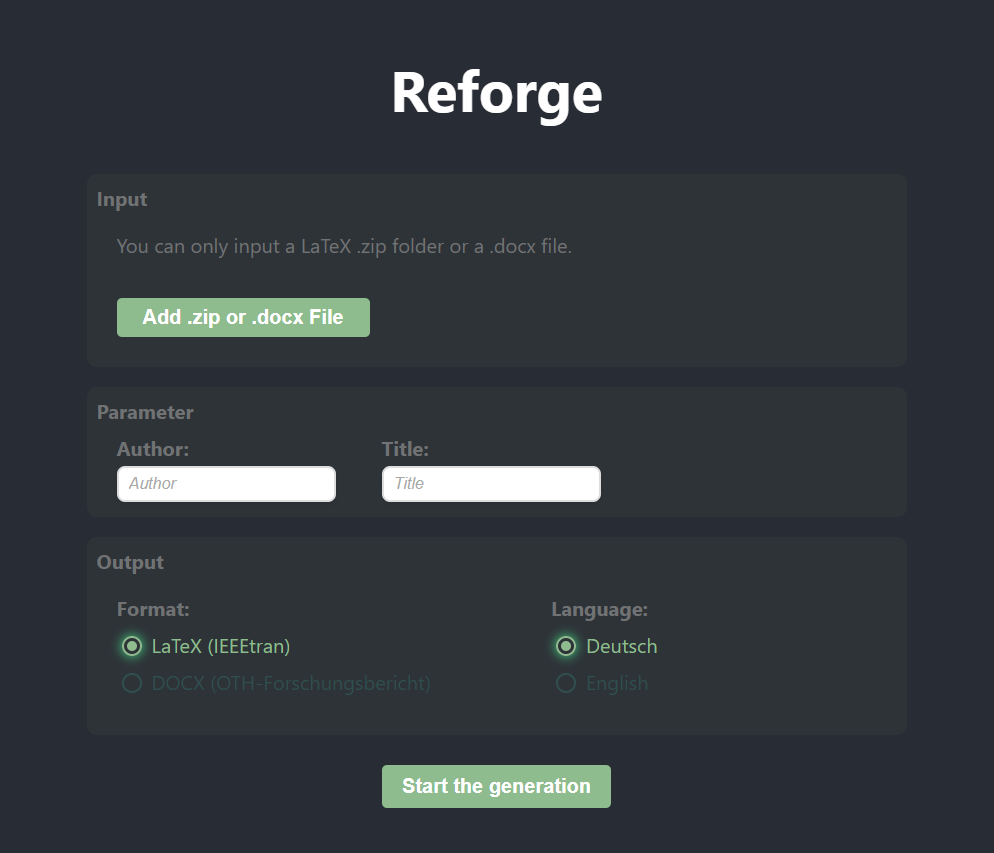
\includegraphics[width=0.9\linewidth]{Images/Frontend Design.png}\\
\caption{Oberflächendesign der Upload-Seite}
\label{fig:Frontend_Design_Upload}
\end{figure}

Die Benutzeroberfläche der Upload-Seite wurde zur besseren Übersichtlichkeit in drei klar definierte Bereiche unterteilt:    
\begin{description}
    \item[Input-Bereich:]
    In diesem Bereich können Dokumente hochgeladen werden, die als Grundlage für die Berichtserstellung dienen. Es werden nur LaTeX-ZIP-Ordner oder \ac{DOCX}-Dateien unterstützt. Diese Einschränkung stellt sicher, dass nur zulässige Dateiformate verarbeitet werden.
    \item[Parameter-Bereich:] 
    Hier werden Parameter wie Autor, Titel und im Falle eines ZIP-Uploads die LaTeX-Hauptdatei eingegeben. Diese Informationen werden für die personalisierte Generierung des Berichts benötigt.
    \item[Output-Bereich:]
    In diesem Bereich kann der Benutzer das gewünschte Ausgabeformat auswählen. Er kann zwischen einer LaTeX- oder einer \ac{DOCX}-Ausgabe entscheiden. Außerdem kann hier die Sprache des Berichts festgelegt werden, wobei der Benutzer nur zwischen Englisch und Deutsch wählen kann.
\end{description}

Die Schaltfläche \textbf{Start the generation} am unteren Rand der Benutzeroberfläche ermöglicht es dem Benutzer, den Prozess der Berichtsgenerierung zu beginnen. Durch die farbliche Hervorhebung ist die Schaltfläche leicht erkennbar und intuitiv zu bedienen.

Die Abbildung \ref{fig:downloadpage} zeigt das Design der Downloadseite. Seit der Erstellung des Wireframes wurden, abgesehen von der Farbgestaltung, keine Änderungen vorgenommen. Lediglich zwei Buttons wurden vorgesehen. Mit \textbf{Download Report} wird der Bericht heruntergeladen und mit \textbf{Generate Another Report} gelangt der Benutzer zurück zur Upload-Seite, falls er einen weiteren Bericht generieren möchte.

\begin{figure}[H]
\centering
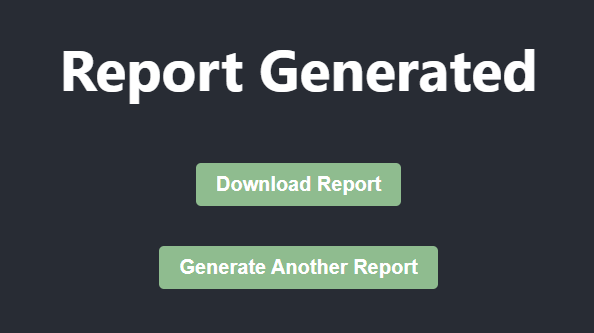
\includegraphics[width=0.5\linewidth]{Images/downloadpage.png}\\
\caption{Oberflächendesign der Download-Seite}
\label{fig:downloadpage}
\end{figure}

Insgesamt wurde bei der Oberflächenentwicklung auf folgendes geachtet:

\begin{description}
    \item[Konsistenz:] Es wurde darauf hingearbeitet, dass die Oberfläche einheitlich ist. Das bedeutet, dass zum Beispiel anklickbare Elemente wie Schaltflächen immer gleich aussehen. So versteht der Benutzer, dass es sich um eine Schaltfläche handelt. Würde man einer Schaltfläche immer wieder eine andere Farbe oder Form geben, wäre dies für den Endnutzer verwirrend. Die Konsistenz hilft, die Bedienung vorhersehbar zu machen.
    
    \item[Feedback und Sichtbarkeit:] Ein weiterer Punkt ist, dem Benutzer ein angemessenes Feedback zu geben, insbesondere wenn er eine falsche Eingabe macht. Wenn der Benutzer beispielsweise vergisst, eine Datei hochzuladen, wird ein Hinweis angezeigt. In diesem Fall werden die Hinweise unterhalb des Start-Buttons angezeigt. Ein Beispiel für eine solche Fehlermeldung ist in Abbildung \ref{fig:Fehleranzeige_Upload} dargestellt. Damit soll der Benutzer bei der Bedienung der Anwendung unterstützt und geführt werden. Sichtbarkeit bedeutet auch, dass der Status des Systems für den Benutzer jederzeit klar sein sollte. Dies wird ebenfalls, wie bei der Fehlermeldung, durch eine Textmeldung an gleicher Stelle erreicht.

    \begin{figure}[H]
    \centering
    
\includegraphics[width=0.8\linewidth]{Images/Frontend_Fehler.png}\\
    \caption{Fehleranzeige auf der Upload-Seite}
    \label{fig:Fehleranzeige_Upload}
    \end{figure}

    \item[Einfachheit und Klarheit:] Die Benutzeroberfläche ist so einfach wie möglich gestaltet. Unnötige Informationen werden vermieden, um den Benutzer nicht zu überfordern. Die Verwendung von klaren Elementen und minimalem Text lenkt die Aufmerksamkeit auf die wesentlichen Funktionen.

    \item[Visuelle Hierarchie:] Durch den gezielten Einsatz von Farben, Größen und Abständen wurde eine klare visuelle Hierarchie geschaffen. Wichtige Informationen oder Aktionen sind hervorgehoben. Dies erleichtert die Orientierung und unterstützt den Benutzer. Auf diese Weise erkennt der Benutzer, was auf der Seite zu erledigen ist. 
\end{description}

Das endgültige Design der Benutzeroberfläche bietet eine klare Struktur, in der die Aufgaben des Benutzers leicht zu verstehen sind. Die gewählten Farben sorgen für eine angenehme visuelle Erfahrung und heben die wichtigsten Aktionen hervor.

\subsection{Die Upload-Seite}
Die Upload-Seite ist, wie bereits erwähnt, dafür verantwortlich, alle für die Berichtsgenerierung notwendigen Informationen an das Backend zu übermitteln. Im Abschnitt \ref{subse:kommu_froback} wurde bereits beschrieben, wie die Kommunikation zwischen Backend und Frontend abläuft. Es wird daher nur auf die zusätzliche Eingabe eingegangen.

Wenn der Benutzer eine ZIP-Datei hochlädt, erscheint ein zusätzliches Eingabefeld. In diesem zusätzlichen Eingabefeld muss der Benutzer den Namen der Hauptdatei des LaTeX-Ordners angeben. Dies wird im Backend dafür benötigt, um die LaTeX-Inhalte in die richtige Reihenfolge zu bringen. Die Abbildung \ref{fig:mainfile_frontend} zeigt, wie das zusätzliche Eingabefeld für die LaTeX-ZIP-Datei aussieht. Wird ein \ac{DOCX}-Dokument hochgeladen, gibt es dieses Eingabefeld für die Hauptdatei nicht, da \ac{DOCX} es nicht benötigt.

\begin{figure}[H]
\centering
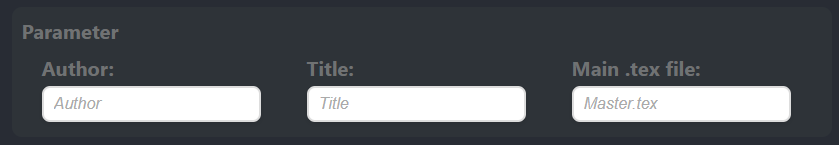
\includegraphics[width=0.8\linewidth]{Images/mainfile_frontend.png}\\
\caption{Das zusätzliche Eingabefeld für die LaTeX-Hauptdatei}
\label{fig:mainfile_frontend}
\end{figure}

\subsection{Die Download-Seite}

Die Download-Seite muss nur die Funktion des Datei-Downloads erfüllen. Die benötigten Daten werden mithilfe des State-Parameters an diese Seite übergeben. Dieser speichert die Zustandsinformationen der aktuellen Seite und ermöglicht deren Übergabe an die Zielseite. Der Wechsel zwischen den Seiten erfolgt über den React Router, der hierfür die Navigate-Funktion nutzt.

Im Listing \ref{lst:state-übergabe} wird der Vorgang der Datenübergabe dargestellt. Dabei wird der React Router verwendet, um die Download-Seite anzusteuern. Der Navigate-Befehl enthält den Zielpfad \texttt{'/download'} und den State-Parameter, der die erforderlichen Informationen wie die Download-\ac{URL}, den Dateititel und das gewünschte Format enthält. Diese Informationen werden anschließend auf der Download-Seite genutzt, um den Download-Prozess auszuführen.

\begin{listing}[H]
\begin{minted}[
frame=lines,
bgcolor=base,
fontsize=\footnotesize,
linenos
]
{typescript}
navigate('/download', { state: { downloadUrl: url, title: title, format: format } });
\end{minted}
\caption{State Übergabe von der Upload-Seite and die Download-Seite}
\label{lst:state-übergabe}
\end{listing}

Der Status der Anwendung wird auf der Download-Seite mit dem \texttt{useLocation}-Hook des React Routers ausgelesen. Die im State enthaltenen Informationen werden über \texttt{location.state} extrahiert. Da das Projekt mit TypeScript umgesetzt wird, müssen die Typen des State-Objekts eindeutig definiert werden. Dies geschieht über das Interface \texttt{LocationState}, welches die Struktur und die Typen der State-Eigenschaften eindeutig beschreibt. Die Implementierung ist im Listing \ref{lst:useLocation} dargestellt.

\begin{listing}[H]
\begin{minted}[
frame=lines,
bgcolor=base,
fontsize=\footnotesize,
linenos
]
{typescript}
import { useLocation } from 'react-router-dom';

interface LocationState {
  downloadUrl: string;
  title: string;
  format: string; 
}

const DownloadPage: React.FC = () => {
  const location = useLocation();
  const { downloadUrl, title, format } = location.state as LocationState;
\end{minted}
\caption{UseLocation-Hook auf der Download-Seite in \textit{Reforge}}
\label{lst:useLocation}
\end{listing}

Um die übergebenen Daten für den Download-Prozess zu verwenden, wird eine Funktion \textbf{handleDownload} implementiert. Diese erzeugt ein temporäres Link-Element, welches die Datei anhand der übergebenen \ac{URL} herunterlädt. Der Dateiname setzt sich dabei aus dem Titel und dem Format der Datei zusammen. Nach dem Klick auf das erzeugte Linkelement wird dieses wieder entfernt, um keine unnötigen Elemente im \ac{DOM} zu hinterlassen. Listing \ref{lst:handleDownload} zeigt, wie diese Funktion realisiert wird. Diese Methode stellt eine Möglichkeit dar, Dateien im Browser herunterzuladen.

\begin{listing}[H]
\begin{minted}[
frame=lines,
bgcolor=base,
fontsize=\footnotesize,
linenos
]
{typescript}
  const handleDownload = () => {
    const link = document.createElement('a');
    link.href = downloadUrl;
    link.setAttribute('download', `${title}.${format}`); 
    document.body.appendChild(link);
    link.click();
    link.remove();
  };
\end{minted}
\caption{HandleDownload-Funktion auf der Download-Seite}
\label{lst:handleDownload}
\end{listing}
